\section{Conceptual Idea}

Haikunet is a SDN programming langauge which was created with the main objective of fulfilling the need of debugging the network, and creating an intent's oriented programming language agnostic to the controller. This last property means that Haikunet will not be coupled to a particular controller at all. Right now OpenDayLight and ONOS are the Controller's supported, but as you will see in following sections, enlarge this number is not hard at all, and you will have the chance to do this by following the tutorial.\\
Writing programs in Haikunet is really easy and straightforward, and this language will give you the advantage of having just one intent written in a common way for several controllers, something that up to now you weren't able to do as far as the writers of this thesis know.\\
The language is interpretated, written in Ruby and can be ran in any machine with a Ruby major or equal version of 2.0.0. This is how a program written in Haikunet looks like:

\begin{lstlisting}[language=Ruby,breaklines=true]
one_host := Host(mac="9A:4A:43:D4:36:45", vlan="-1", ipAddresses=["10.0.0.1"], elementId="of:0000000000000002", port="4")

second_host := Host(mac="72:D2:0D:24:C5:36", vlan="-1", ipAddresses=["10.0.0.4"], elementId="of:0000000000000003", port="4")

my_flow := Flow (src=one_host, dst=second_host, priority="55")

Intent firstExample
	Select my_flow
\end{lstlisting}

This program describes an intent for creating a flow between two host. We will come back to explain in more detailed this program and all the elements involve in the \textbf{Learning Haikunet} section.\\

The main ideas that you have to understand before writing a program in this language are the followings:

\begin{itemize}
\item Initial Topology\\
Which would be the initial topology?, think of this as the network in which you want to apply the intent. It's called initial because it can be seen as the initial point from where we start, and after the intent is applied to the newtork, we will obtain the desired network, which can be called the last one. In the \textbf{Formal Definition} section this is better explained.
\item What is what you want from the newtork?\\
Try to understand well what are you going to ask to the network, if it's possible to do it, which components are going to be involved in, etc. From this though, you will write your program.
\item Which is going to be the destiny?\\
Has the destiny the ability to do what you are expecting from the network?. Remember that you can always debug first what you are doing, and then proceed to apply it to the real network!.
\end{itemize}

After this, as every programming language, you will need to practice in order to write good programs. Let's take a look at the architectural components of the language, and how they relate one with each other.

\begin{figure}[H]
\centering
\includegraphics[width=\textwidth]{images/haikunet/arquitectura_haikunet.png}
\caption{Haikunet architectural view}
\end{figure}

The components in the left are the arguments the interpreter expect (except the topologygenerator tool which is a gem used by the language). We will come back in more detailed to these arguments in the \textbf{Learning Haikunet} section.\\
Inside the black box are the components which make up the interpreter, these will be explained in more detailed at the \textbf{Implementation} section, and finally at the right are the possible outputs that the language can provide (ONOS and OpenDayLight component's represent a generation of a bunch of request to one of these controllers, DEVS is the generation of the .pdm file, and finally ERROR represents that something went wrong while interpretating the program). These will also be seen in the \textbf{Learning Haikunet} section.\\

As it can be apreciated in the image, Haikunet uses the topologygenerator tool which was explained in the previous chapter. The topologygenerator gives an important characteristic to the language, which is that it allows us to create a NTM model and use it as our intial network, meaning that it's not mandatory to have a real network for using Haikunet. Another important thing is one of the destinies which Haikunet support's, DEVS. Supporting this destiny gives the language an important characteristic, which is permiting to simulate from either a real network or a NTM model how would an intent react in the initial newtork.\\

Haikunet flow's work as follow: We first run the interpreter giving as argument a progam and an output destiny, this output destiny specifies to which controller the program is being interpretated. The interpreter lexer's then receive the program, which will be in charge of tokenize it and give it to the parser, which will detect if the tokens are gramatically well written. After this, the semantic checker will detect either statical or dynamical errors in the program (we will explain in more detailed this erros definition's in the \textbf{Formal Definition} section), using the underlaying network which was given by the topologygenerator tool. After this two things can happen: either the program had no errors, meaning that the code generator will execute the bunch of request that have to be done to the API of the controllers specified in the input of the interpreter, or it had, this will cause an error raise exception with a message which will explain the problem. \\

This short paragraph resumes the working flow of a program being interprated by Haikunet. In the \textbf{Language Implementation} section we will cover in detailed what happens in each of the components previously mentioned.\\

Now that we have a better idea of what Haikunet is, let's proceed to give some formal definition's before getting into the tutorial, but before this let us explain you something.

\section{Why Haikunet?}

The name Haikunet comes from the join of Haiku and Network. A Haiku is a Japanese poem with a lot of themes, but in most of the cases a Haiku describes the nature from the view of an observer. This is exactly what you are going to do with Haikunet, write short programs which will describe the desired nature of a network, and this description will be done from the point of view of an observer of the network, meaning a person which does not necessarily knows how to interact at a system level with it, and in most of the cases, doesn't know how to. This is the intent's programmer point of view of the network. 

\section{Formal Definition}

In this section we will establish key concepts and main ideas that will be use in this chapter. The section will be divided in one definition after another, and after all definitions are made, we will continue with the Haikunet tutorial.\\

\subsection{Debugging}

Debugging will be the process of finding either static or dynamic errors before the intent is applied to the network. The definition of these type of erros can be found ahead in the section.\\
In this work, we are not going to explore techniques which involves stopping an intent execution's in a controller. 

\subsection{Error}

An error will be a request made by a program written in Haikunet, which has not semantically sense in the context of the current network. Since this definition involves a huge amount of errors for a thesis work, we will focus in a limited scope which will be introduced next. We will show some scenarios, their respectively errors in them, and the error output that the interpreter will show:

\subsubsection{Flow property definition error}

\textbf{Description:} This error happens when you use a host property in a flow definition, and this property cannot be neither found or inferred from the initial network topology. \\

\textbf{Example:} Let's suppose that we have the following initial network:

\begin{figure}[H]
\centering
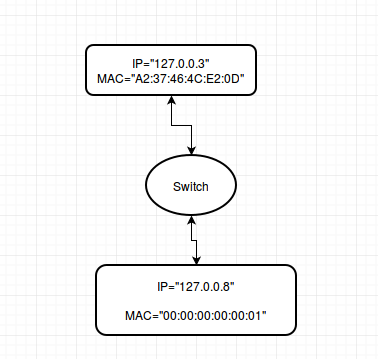
\includegraphics[width=\textwidth]{images/haikunet/error_scenario_1.png}
\caption{Initial network context in flow property definition error}
\end{figure}

and we execute the following program:

\begin{lstlisting}[language=Ruby,breaklines=true]
source_host := Host(mac="A2:37:46:4C:E2:0D")

my_flow := Flow (src=source_host, dst="127.0.0.10", priority="55")

Intent firstExample
    Select my_flow
\end{lstlisting}

In this example, we have the problem that the property \textit{dst = "127.0.0.1"} is not a valid ip in the current network. \\

An important observation here is that this is an error, because the mistake is made in the flow definition line. If we would have a mispelled property in the Host definition as we show in this example (let's assume that I wanted to create a flow between \textit{127.0.0.3} and \textit{127.0.0.8}):

\begin{lstlisting}[language=Ruby,breaklines=true]
source_host := Host(ip="127.0.0.2")

my_flow := Flow (src=source_host, dst="127.0.0.8", priority="55")

Intent firstExample
    Select my_flow
\end{lstlisting}

This would not be considered as an error, since the semantic of this program in the initial network context given before, would mean first to create a host with \textit{127.0.0.2} as IP, and then create a flow between this new host and the one which has \textit{127.0.0.8} as IP.

\subsubsection{No path error}

\textbf{Description:} This error is thrown when you are trying to create a flow between two host which have no path between them.

Let's suppose that we have the following initial network:

\begin{figure}[H]
\centering
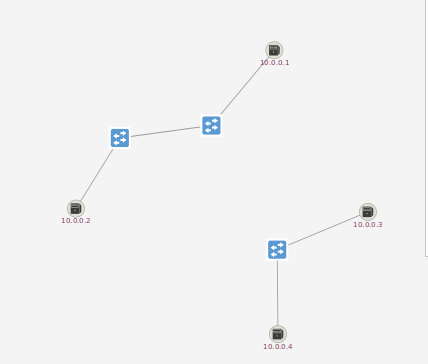
\includegraphics[width=\textwidth]{images/haikunet/error_scenario_2.png}
\caption{Initial network context in no path error}
\end{figure}

and we execute the following program:

\begin{lstlisting}[language=Ruby,breaklines=true]
source_host := Host(ip="10.0.0.2")

    destiny_host := Host(ip="10.0.0.4")

my_flow := Flow (src=source_host, dst=destiny_host, priority="55")

Intent firstExample
    Select my_flow
\end{lstlisting}

It can be seen in the image above that the error is thrown because there is no path between hosts \textit{10.0.0.2} and \textit{10.0.0.4}. 

\subsubsection{Inconsistent host definition error}

\textbf{Description:} This error is thrown when you are trying to either create or refer to a Host which already exist with different properties from the real ones. 

Let's suppose that we have the following initial network:

\begin{figure}[H]
\centering
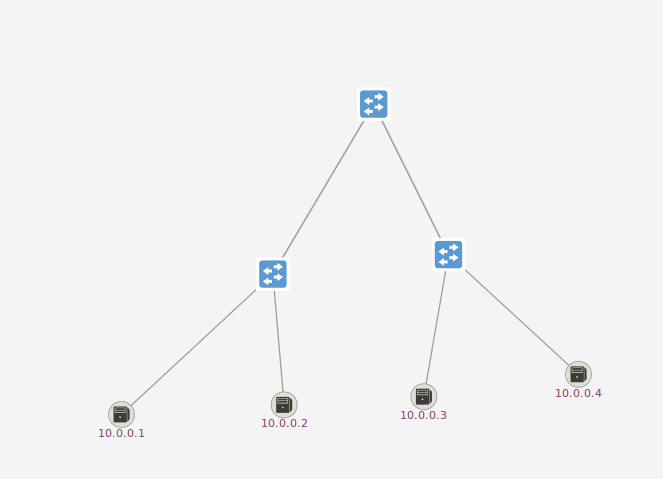
\includegraphics[width=\textwidth]{images/haikunet/error_scenario_3.png}
\caption{Initial network context in inconsistent host definition error}
\end{figure}

and we execute the following program:

\begin{lstlisting}[language=Ruby,breaklines=true]
one_host := Host(mac="9A:4A:43:D4:36:45", vlan="-1", ipAddresses=["10.0.0.1"], elementId="of:0000000000000002", port="1")

second_host := Host(mac="72:D2:0D:24:C5:36", vlan="-1", ipAddresses=["10.0.0.4"], elementId="of:0000000000000003", port="2")

my_flow := Flow (src=one_host, dst=second_host, priority="55")

Intent firstExample
    Select my_flow
\end{lstlisting}

The problem here is that we are trying to define the same host with different mac addresses. CORRECT THE IMAGE SO WE CAN SEE THE HOST WITH ITS CURRENT MAC.

\subsubsection{Percentage in loss packets error}

STILL HAS TO BE IMPLEMENTED.

\subsection{Static and Dynamic errors}

When debugging definition was made, static and dynamic errors were mentioned. We now proceed to define each type of error, and we will categorize the erros showed before in order to understand better these definitions.

\begin{itemize}

\item Static error\\
A static error can be defined as an error which can be pointed out as one, without the need of letting time pass into the underlying network. Examples of these types of erros showed before are the \textit{Flow property definition error}, \textit{No path error} and \textit{Inconsistent host definition error}
\item Dynamic error\\
A dynamic error can be defined as an erorr which needs time to be elpased in the underlying network, in order to identify it as one. An example of this kind of error is the \textit{Percentage in loss packets error}. 
\end{itemize} 

As it can be seen on the definition above, time is a variable needed for defining both kind of errors. This variable is introduced because the network is a model which is always changing, and not necesarilly just because a program changes it (for example we can always have either infraestracture or software issues, making links and host not reacheable, causing a change in the underlying network topology).\\
From the definition of both types of erros, we studied the best way to detect each of them.\\
From the first type of errors, an interpreter using a network model plus a definition of a semantic checker were implemented in order to detect them.\\ Since for detecting the second type of errors we need time to be elapsed in the underlying network, and the time needed varies depending on each error, a connection with DEVS was implemented. The key idea in this is having a representational model of the network, which can be ran as a simulation in DEVS, modelling hours of time elapsed in the network. The simulation will then replied with results, and from this results we will be able to detect if there are dynamic errors present in the program. 


\subsection{Initial Network}

The concept of initial network comes from the following view: When you apply an intent to a network, you can see the network as a mutable element which is being transformed by the application of an intent. This abstraction allow us to identify different network states that can be pointed out in the intents process: The first one, the initial one, is the network in which the user wants to apply the intent. Then there is a last one, which is the one in which the intent has already been applied, in case it was possible to do so, and is the newtork result of applying the intent. Since the intent can transform several times the network (for example first adding a host, then adding a link, etc.), we can identify all the intermediate states in which the network has to be in order to reach the last state. \\
From the given approach, in the \textbf{Future work} section we will introduce several ideas that we have related to this important concept.

\section{Tutorial}

\subsubsection{Installation}

\textbf{Pre-requisite:} You need to have a git client installed, a machine running a Linux distribution (it was tested in an Ubuntus machine, but should work in any Linux distribution machine), and already installed a ruby version equal or major to 2.0.0.

For installing Haikunet, just run the following commands:

\begin{lstlisting}[language=bash,breaklines=true]
$ git clone git@github.com:andyLaurito92/haikunet.git
$ cd haikunet
$ sudo ./install_haikunet.sh 
\end{lstlisting}

And that's it!, you have already installed the interpreter. Let's understand a bit more about the language before jumping into the code.

\subsubsection{Using the interpreter}

\textbf{Pre-requisite:} Have running locally the ONOS controller, and have already download the language repository.

For running the Haikunet interpreter, you will need: 
\begin{itemize}
\item The path to the file where the haikunet program is (remember that only files with the ".hk" extension are allowed).
\item Specify one of the destinations supported (the current supported are \textit{ONOS}, \textit{OPENDAYLIGHT} and \textit{DEBUG}).
\item An URI from where to obtain the initial topology.
\end{itemize}

Let's get into more detailed in the last two arguments.\\
The destination argument is an option which will tell the interpreter to which destiny has to generate the code of the input program, the options current supported are \textit{ONOS}, \textit{OPENDAYLIGHT} and \textit{DEBUG}. The first two are controllers, and selecting one of them will generate a bunch of request to the corresponding API REST. The DEBUG option will generate a simulation in DEVS, taking as initial topology the one specified by argument, and will show you simulations result's once the run is complete. The idea is that with this results, you will be able to identify if the network behaviour is the one you expected. We will get into more detailed on this in the \textbf{Implementing your first program} subsection.\\
The other argument is the URI from the Initial Network, which was already explained in the \textbf{Formal Definition} section. As the name remarks, will be either a URI of an API REST of a controller, or a path to a file which will contain a ruby NTM (this was explained in the previous chapter, in the \textbf{Network Topology Model} section).\\

Let's now suppose that:
\begin{itemize}
\item We want to execute the \textit{host\_to\_host.hk} program (you can find it in \textit{\$HAIKUNET\_DIRECTORY/examples/programs}), which creates two host if they don't exist in the underlying network, and creates a flow between them. 
\item We are using ONOS as destiny output.
\item We will use as initial topology the one that we have at ONOS. 
\end{itemize} 

This is how you use the interpreter for doing that (we will assume that you will execute the haikunet interpreter from the \textit{\$HAIKUNET\_DIRECTORY}, and the ONOS local version that you are running can be located at http://127.0.0.1:8181 address):

\begin{lstlisting}[language=bash,breaklines=true]
$ haikunet program -n examples/programs/host_to_host.hk -d ONOS -u http://127.0.0.1:8181/onos/v1/
\end{lstlisting}

In the previous command:
\begin{itemize}
\item \textbf{-n} is the option to provide the path to the interpreter.
\item \textbf{-d} is the destiny name.
\item \textbf{-u} is the path to the uri initial topology.
\end{itemize}

If you want to debug the same program using the same initial topology, just run the following command:

\begin{lstlisting}[language=bash,breaklines=true]
$ haikunet program -n examples/programs/host_to_host.hk -d DEBUG -u http://127.0.0.1:8181/onos/v1/
\end{lstlisting}

You may also want to try to use as initial topology the one provided in \textit{examples/initial\_topologies} to debug it. The command to run in this case is:

\begin{lstlisting}[language=bash,breaklines=true]
$ haikunet program -n examples/programs/host_to_host.hk -d DEBUG -u examples/initial_topologies/example_topology.rb
\end{lstlisting}

In case your default controller is OpenDayLight, you just have to use the OPENDAYLIGHT destiny, and specify the uri \textit{http://OPEN\_DAY\_LIGHT\_IP:8080/restconf/operational/network-topology:network-topology/topology/flow:1/}, where \textit{OPEN\_DAY\_LIGHT\_IP} stands for the corresponding IP address of the controller. 

You can find these and more examples in the interpreter help's by running the following command:

\begin{lstlisting}[language=bash,breaklines=true]
$ haikunet program --help
\end{lstlisting}

Now that we know how to use the interpreter, let's write our first program!.

\subsubsection{Implementing your first program}



\section{Language Implementation}

\subsection{Lexer/Parser}

\subsection{Semantic Checker}

\subsection{Code Generation}

\section{Implementing your CodeGenerator}

\section{Limitations}

\section{Future work}